\documentclass[10pt,draftclsnofoot,onecolumn]{IEEEtran}

\usepackage{listings}
\usepackage{graphicx}

\graphicspath{ {images/} }
\title{Group 07, GTA Corvallis Final Report}
\author{Jonah George, Kris Vand Zandt, and Ryan Graysmark}
\date{March 2016}

\lstset{ %
  basicstyle=\footnotesize,        % the size of the fonts that are used for the code
  breakatwhitespace=false,         % sets if automatic breaks should only happen at whitespace
  breaklines=true,                 % sets automatic line breaking
  frame=single,	                   % adds a frame around the code
  keepspaces=true,                 % keeps spaces in text, useful for keeping indentation of code (possibly needs columns=flexible)
  language=Ruby,                 % the language of the code
  numbers=left,                    % where to put the line-numbers; possible values are (none, left, right)
  tabsize=2,	                   % sets default tabsize to 2 spaces
}

\begin{document}

\maketitle

\hfill \break \hfill \break \hfill \break
\hfill \break \hfill \break \hfill \break
\hfill \break \hfill \break \hfill \break
\hfill \break \hfill \break \hfill \break

\begin{abstract}
The GTA Corvallis project has almost completed all of our system requirements that we set in the Fall of 2015.
Admins are now able to run the ILP which uses the constraints that we have defined to select the best student to the right class.
With some last minute changes before expo, the project will be fully completed.
\end{abstract}

\pagenumbering{gobble}% Turn off page numbering.
\newpage
\pagenumbering{arabic}% Turn page numbering back on.

\section{Introduction}

\subsection{Problem Statement}

GTA Corvallis is a project sponsored by Prasad Tadepalli of the OSU Computer Science department. Currently, Professor Tadepalli is responsible for hand-assigning graduate teaching assistants (GTAs) to classes at the beginning of each term. This takes an unreasonable amount of time and can be very frustrating when dealing with the requests of numerous instructors and students. 

\subsection{Proposed Solution}

Our proposed solution is to build a web service that will automate the assignment of GTAs to classes. 
Our program will take in many factors such as: student experience, student preferences, teachers preferences, and required skills. 
Our program will also fetch class statistics for all of the classes offered at Oregon State University. 
This means we will always have up-to-date information on class metadata, such as enrollment, capacity, and location. 
Our system relies on students and teachers inputting a variety of information which will help with selecting the right GTA for the right class.


\section{Current Progress}

\subsection{Home Page}

\begin{figure}[htbp]
  \centering
  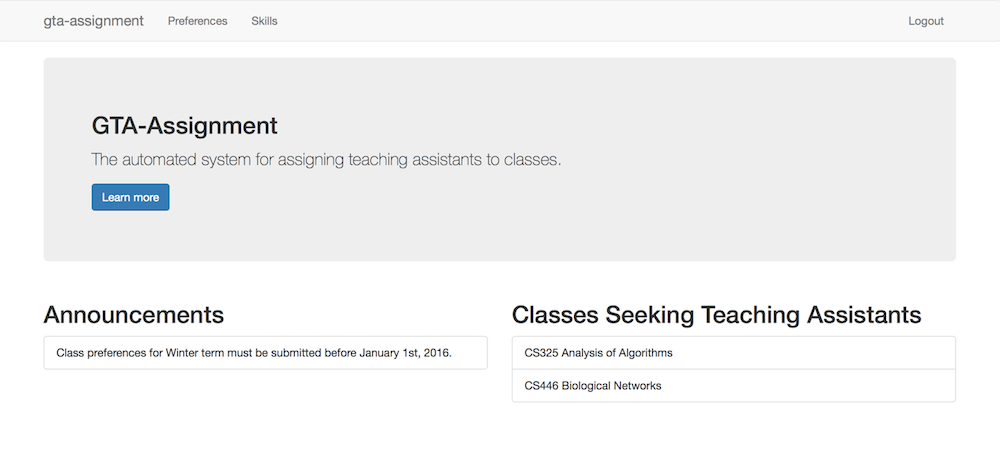
\includegraphics[width=0.75\linewidth]{images/homepage-design.png}
  \caption{Mock Homepage}
\end{figure}

\begin{figure}[htbp]
  \centering
  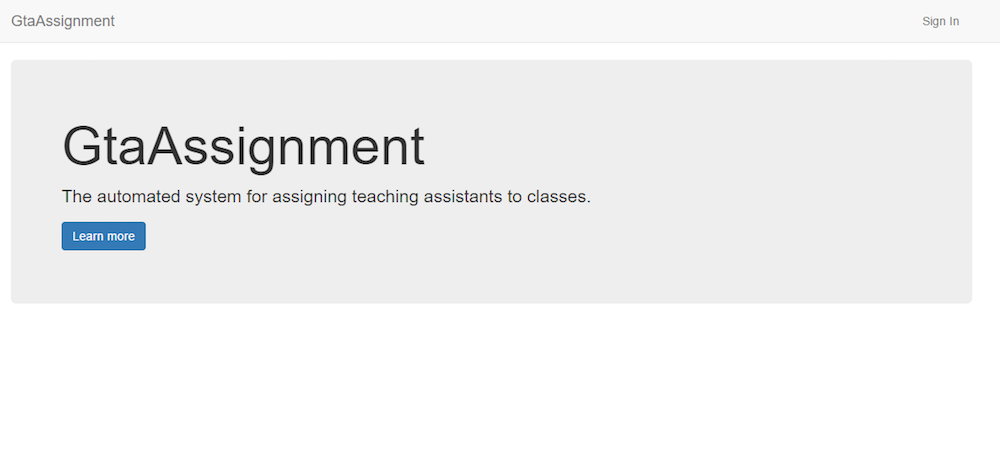
\includegraphics[width=0.75\linewidth]{images/homepage-alpha.png}
  \caption{Alpha Homepage}
\end{figure}

\begin{figure}[htbp]
  \centering
  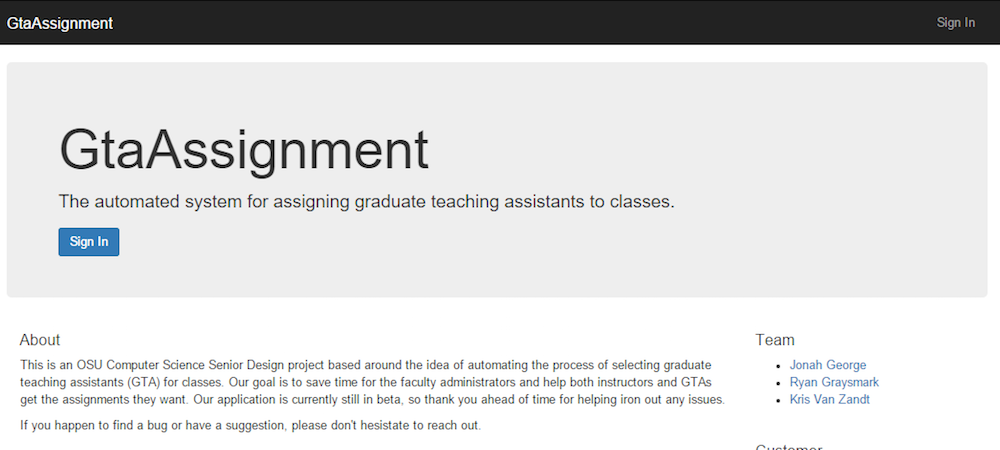
\includegraphics[width=0.75\linewidth]{images/homepage-beta.png}
  \caption{Release Homepage}
\end{figure}

Comparing what we had for our Alpha and what we have for Release, you can see that we fully wrote an 'About' and 'Learn More' section.
Those two sections have replaced the 'Announcements' and 'Classes Seeking Teaching Assistants' which we had from our design document.
These sections give a concise look into our project for anyone who has neveer seen or heard of the site before.
One can also see that at the top right we have the Sign In button, which is configured to log users in with Google OAuth2.
We have also been able to configure the integration to only grant access to users with a Oregon State ONID accounts.

\subsection{Students}

A brief reminder of what some of the tasks a user is supposed to perform includes inputing student preferences and selecting skills.
These will be converted into integer equivalences to be used by our ILP when it is time to assign students to classes.
Students self input all of their information, but we allow admins to be able to edit this information when they see fit.
Our hope is the students know what they are capable of teaching which means knowing the skills and languages they possess along with the classes they would like to teach.

\subsubsection{Student Experience Interface}

\begin{figure}[!htb]
  \centering
  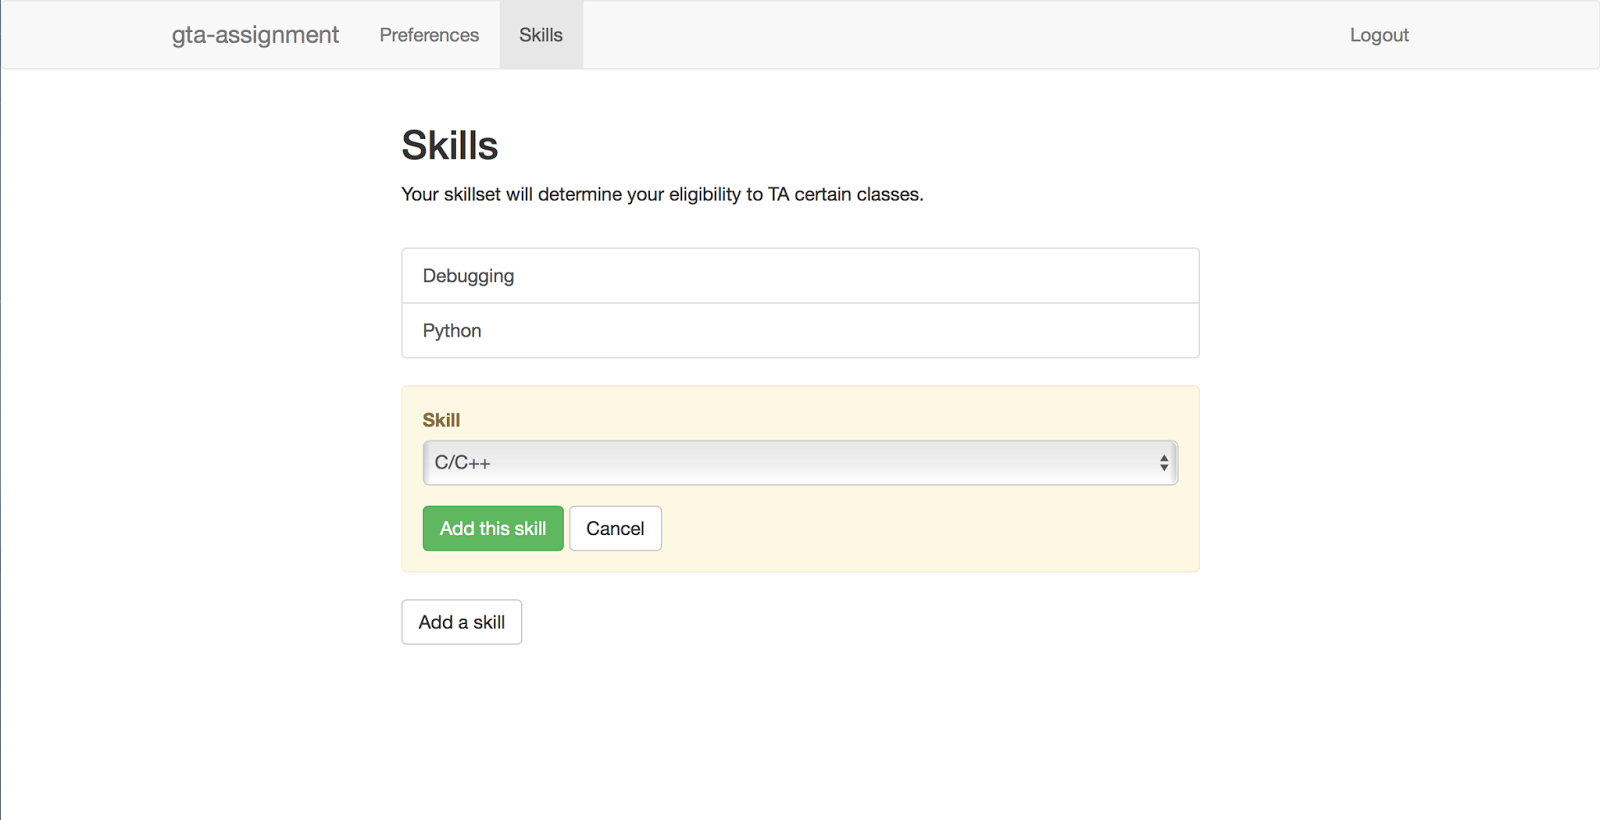
\includegraphics[width=0.75\linewidth]{images/student-experience-design.png}
  \caption{Mock Student Experience Interface}
\end{figure}
\begin{figure}[!htb]
  \centering
  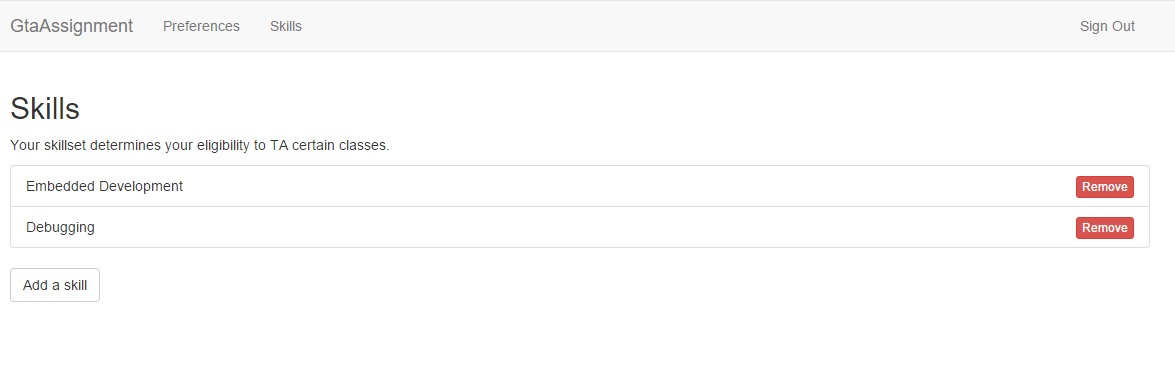
\includegraphics[width=0.75\linewidth]{images/student-experience-alpha.png}
  \caption{Alpha Student Experience Interface}
\end{figure}
\begin{figure}[!htb]
  \centering
  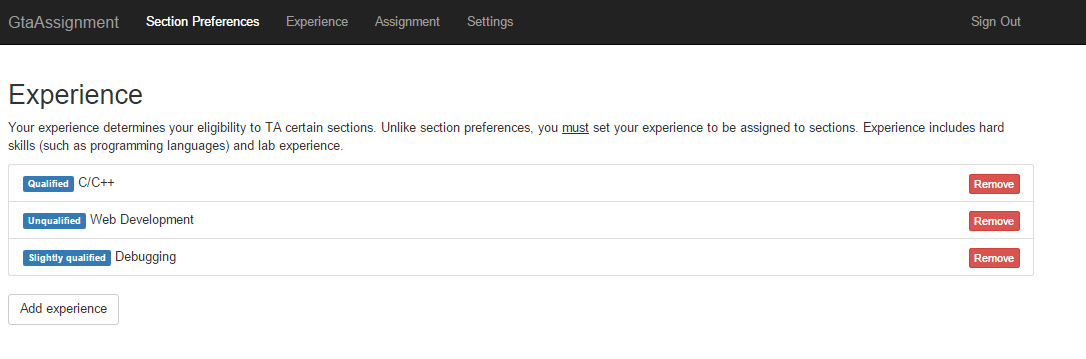
\includegraphics[width=0.75\linewidth]{images/student-experience-beta.png}
  \caption{Release Student Experience Interface}
\end{figure}

% \begin{figure}[!htb]
%   \centering
%   \minipage{0.5\textwidth}
%     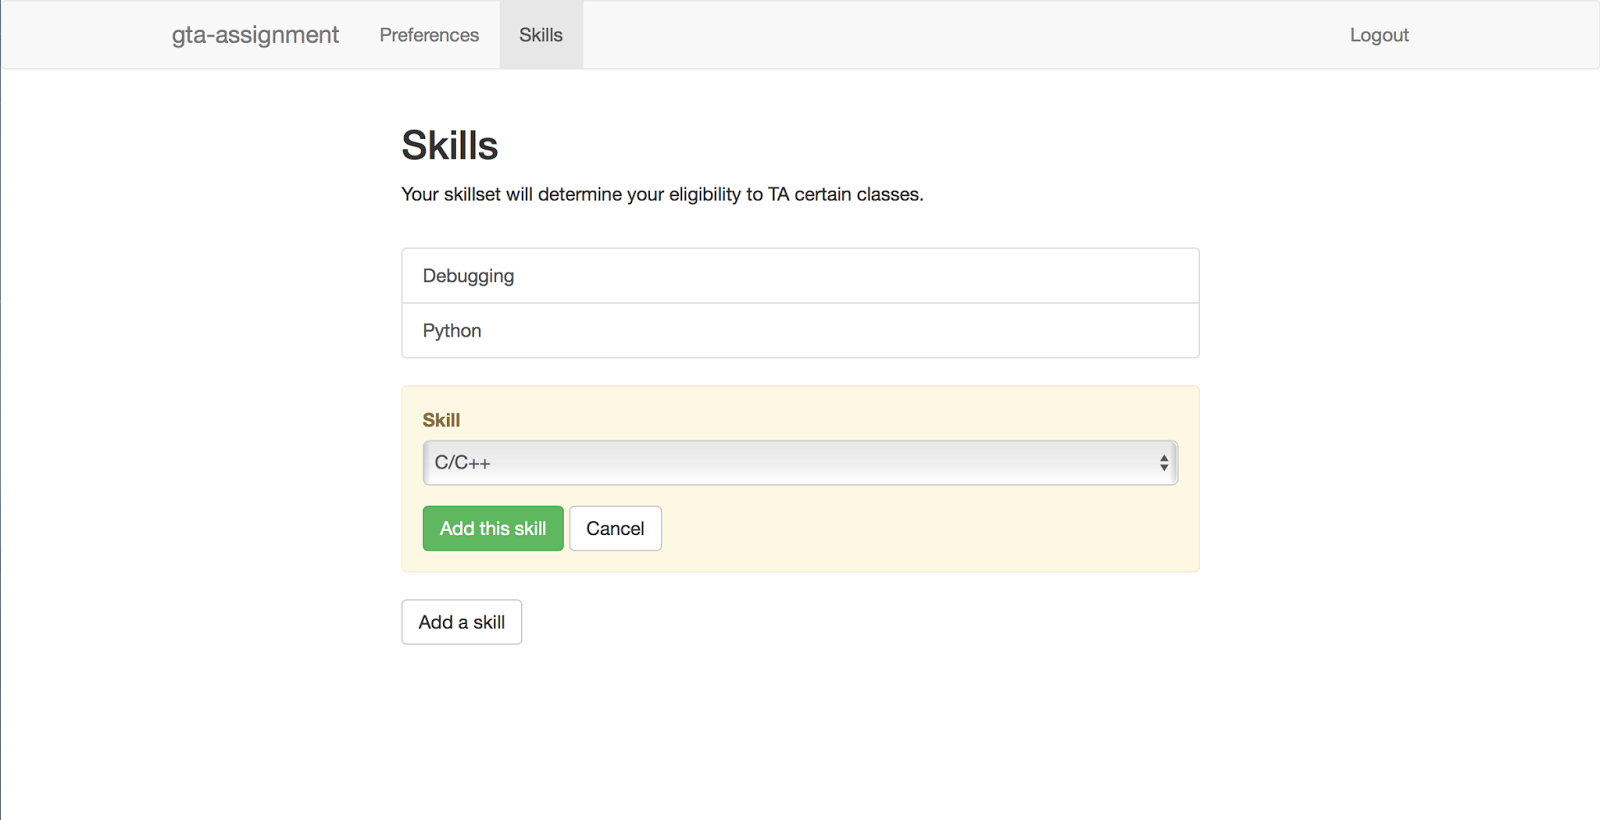
\includegraphics[width=\linewidth]{images/student-experience-design.png}
%     \caption{Mock Student Experience Interface}
%   \endminipage\hfill
%   \minipage{0.5\textwidth}
%     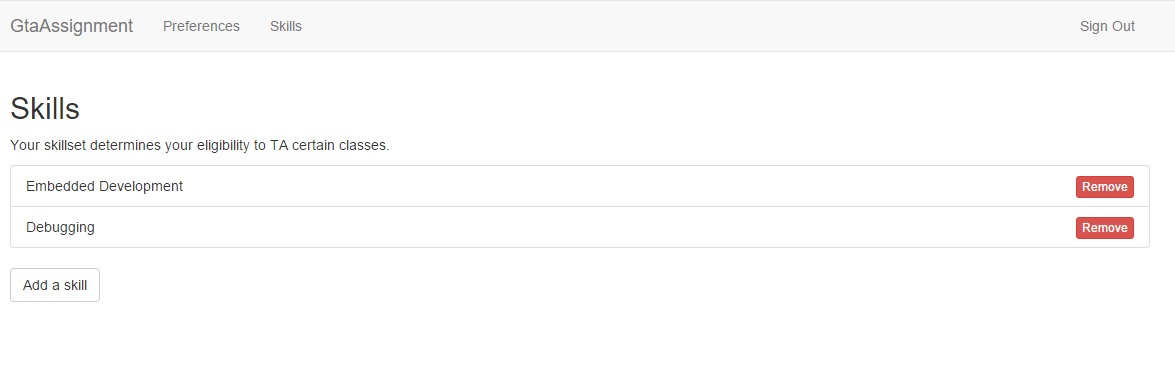
\includegraphics[width=\linewidth]{images/student-experience-alpha.png}
%     \caption{Alpha Student Experience Interface}
%   \endminipage\hfill
%   \minipage{0.5\textwidth}
%     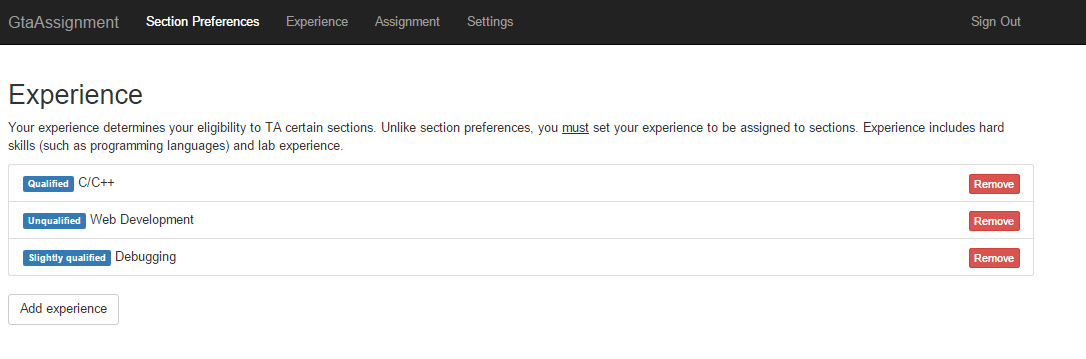
\includegraphics[width=\linewidth]{images/student-experience-beta.png}
%     \caption{Release Student Experience Interface}
%   \endminipage\hfill
% \end{figure}

This section hasn't changed much on the surface from what he had back in Fall - we added a few of sentences describing our project for those who had never used the site before.
The primary changes were on the backend.
After talking with our sponsor we felt that we should focus on combining skills and experience in one super section.
Skills acquired through school might have been acquired differently than a graduate student's experience outside of school yet, they both hold the same fundamental value within the ILP.

\begin{figure}[!htb]
   \centering
   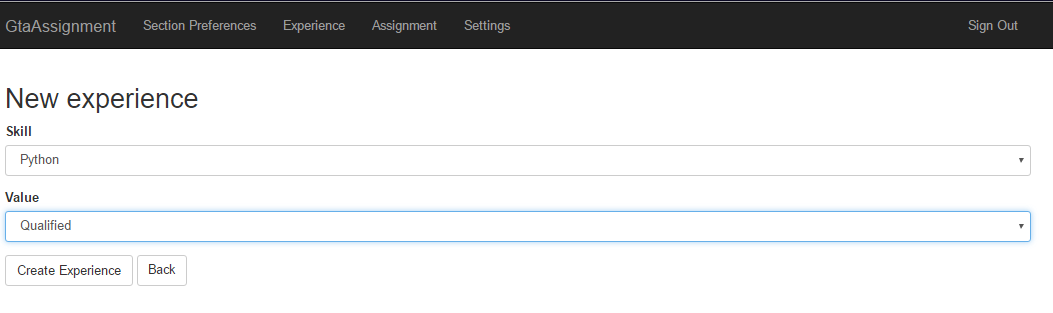
\includegraphics[width=0.75\textwidth]{images/student-new-experience-beta.png}
   \caption{How Students Add Experience From Pre-Defined List of Skills}\label{student-new-experience-beta}
\end{figure}

In Figure \ref{student-new-experience-beta}, one can see that the skill bar is a dropdown which has a list of predefined skills and experience.
With the help of our sponsor we came up with a default list that consists of skills such as python, C, C++, web development, debugging, and many more.
However, if an instructor doesn't see a skill they require, they can always add it via the instructor interface.
Each skill is associated with a student, for as long as they are a TA at Oregon State.
We allow students to select as many skills as they want.
The value that you see ranges from qualified, slightly qualified, to unqualified, where the default value are set to unqualified.
We are giving the power to the students to select the exact skills and experiences that they possess.
This selection is very important to us as it is programmed as a hard constraint in the ILP.
If a student does not have the right skills than they will not be eligible to teach the class.

\subsubsection{Student Preferences}

Student preferences are a key component of the ILP because the goal is to put students in classes they would want to teach.
Currently, we allow the students to select up to 5 classes that they favor or disfavor.
Almost as important as a class a student favors, what a student disfavors can be just as valuable.

\begin{figure}[!htb]
  \centering
  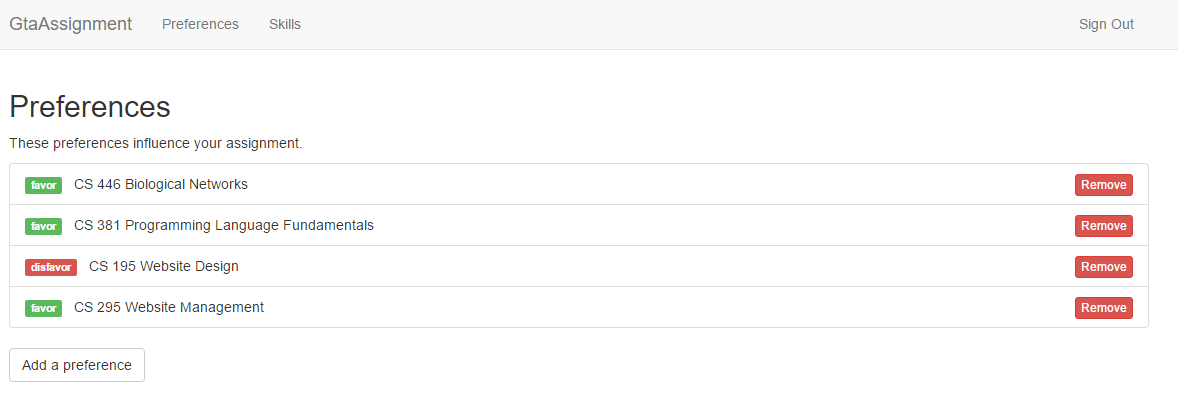
\includegraphics[width=0.75\linewidth]{images/student-preferences-alpha.png}
  \caption{Mock Student Preferences Interface}
\end{figure}
\begin{figure}[!htb]
  \centering
  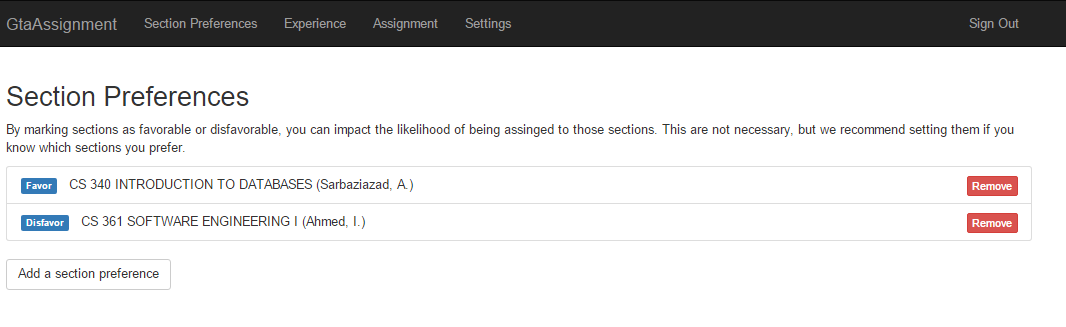
\includegraphics[width=0.75\linewidth]{images/student-preferences-beta.png}
  \caption{Release Student Preferences Interface}
\end{figure}

% \begin{figure}[!htb]
%   \centering
%   \minipage{0.5\textwidth}
%     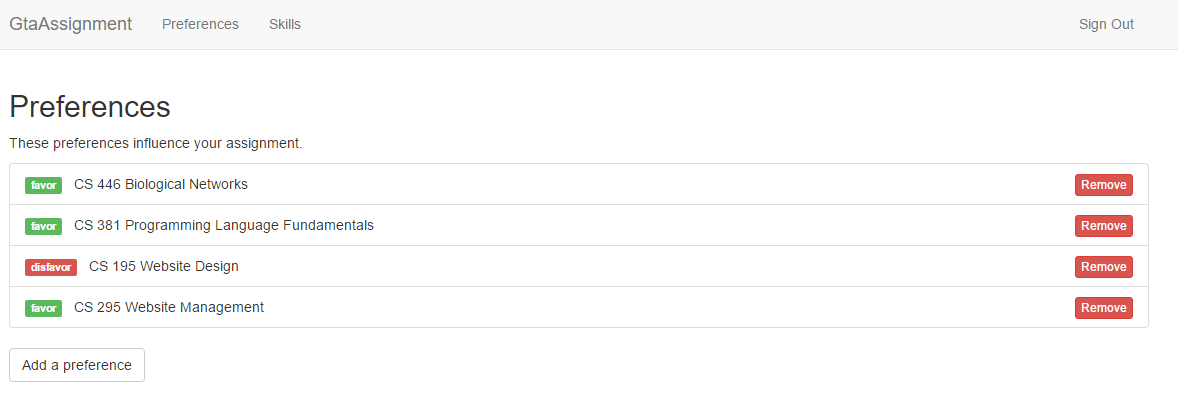
\includegraphics[width=\linewidth]{images/student-preferences-alpha.png}
%     \caption{Mock Student Preferences Interface}
%   \endminipage\hfill
%   \minipage{0.5\textwidth}
%     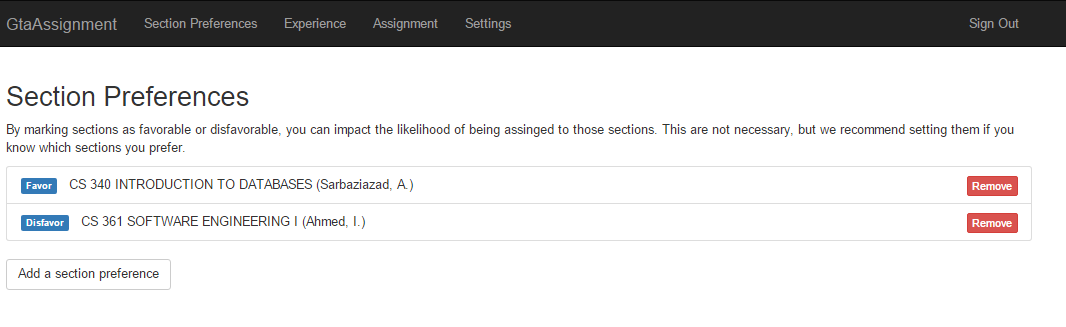
\includegraphics[width=\linewidth]{images/student-preferences-beta.png}
%     \caption{Release Student Preferences Interface}
%   \endminipage\hfill
% \end{figure}

Not a lot has changed from what we envisioned in our mock ups, we added a couple of sentences going into detail about how to use the site along with changing some wording.
We moved away from just preferences to section preferences to show that you are preferring actual sections not just classes.
A class could be taught by multiple instructors each with their own section, so denoting that fact helps clear up some confusion.

Jonah created a web scraper which grabs all the current classes along with course section, instructor, and enrollment sizes.
The list of courses will always be up-to-date because of this.
Students are allowed to select as many preferences as they want.
Each preference has an associated value ranging from Favor to Disfavor with neutral being in the middle.
By default, the section preferences are set to neutral.
This means there is an equal possibility that a student can be assigned any class as long as they have the required skills.
The more preferences they fill out, the greater chance of getting the class they desire.

\subsection{Instructor}

Instructors have a lot of responsibility when it comes to selecting students to be TAs for their classes.
They are usually given the final say on all selections, so the power really rests in their hands.
In our project, we focused on letting them decide students they favor or disfavor and selecting the necessary skills needed for their sections.

\begin{figure}[!htb]
  \centering
  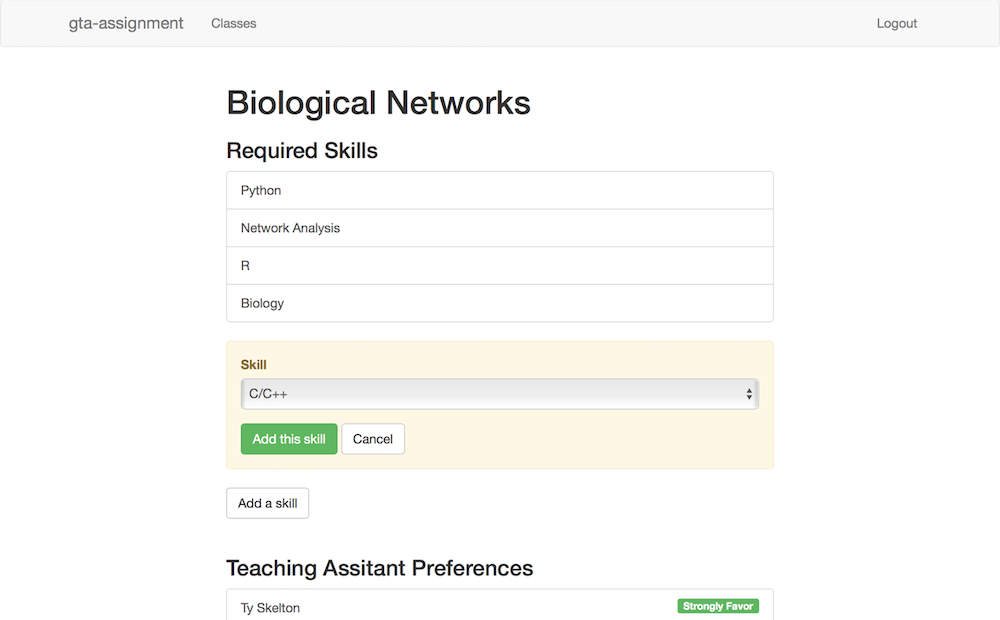
\includegraphics[width=0.75\linewidth]{images/instructor-section-design.png}
  \caption{Mock Instructor Sections Page}\label{instructor-section-design}
\end{figure}

\begin{figure}[!htb]
  \centering
  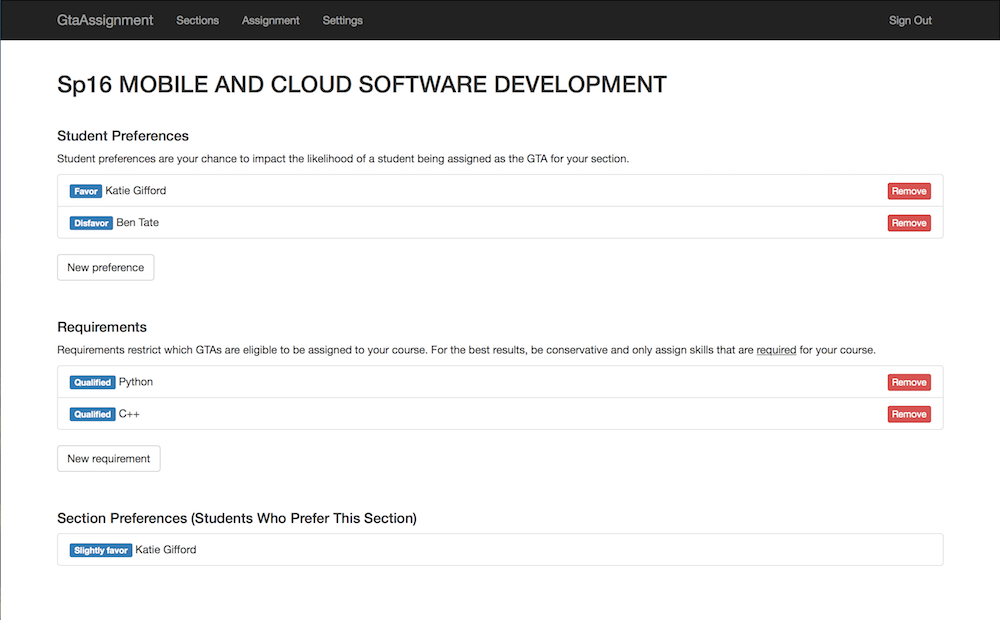
\includegraphics[width=0.75\linewidth]{images/instructor-section-beta.png}
  \caption{Release Instructor Sections Page}\label{instructor-section-beta}
\end{figure}

% \begin{figure}[!htb]
%   \centering
%   \minipage{0.5\textwidth}
%     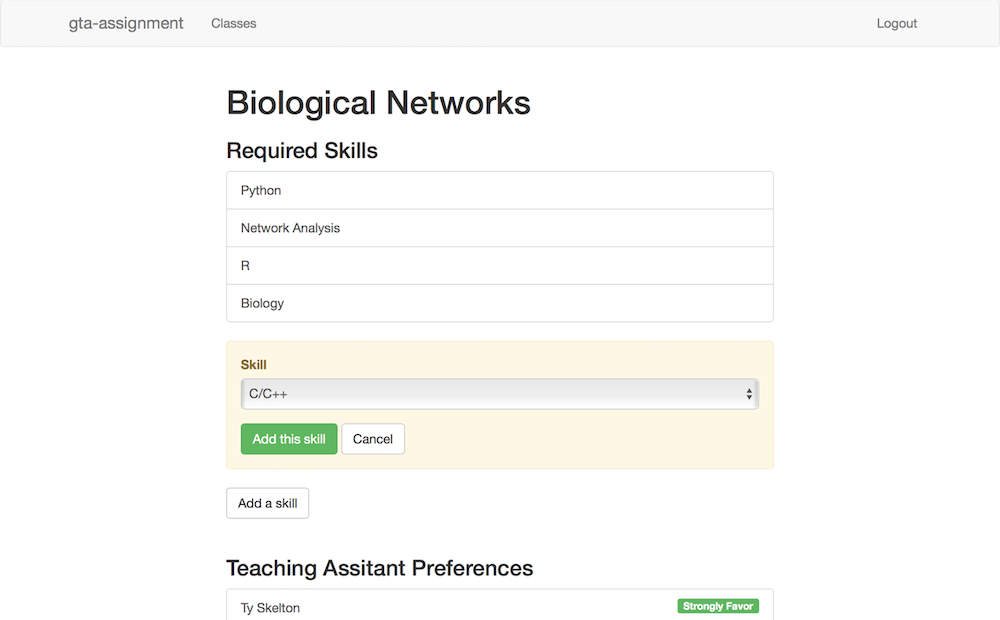
\includegraphics[width=\linewidth]{images/instructor-section-design.png}
%     \caption{Mock Instructor Sections Page}\label{instructor-section-design}
%   \endminipage\hfill
%   \minipage{0.5\textwidth}
%     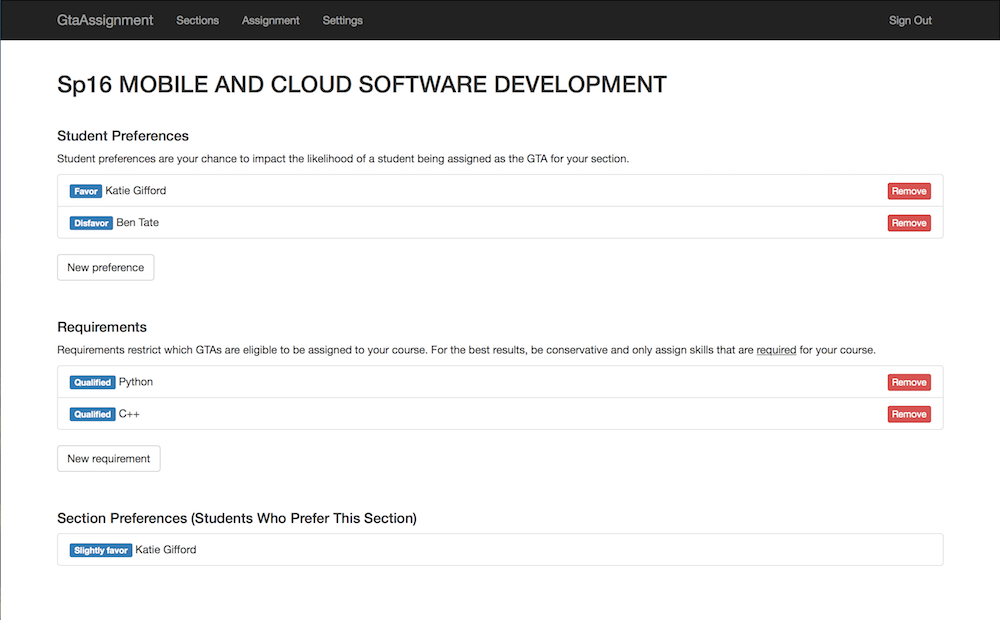
\includegraphics[width=\linewidth]{images/instructor-section-beta.png}
%     \caption{Release Instructor Sections Page}\label{instructor-section-beta}
%   \endminipage\hfill
% \end{figure}

As you can see, we split the classes into sections.
Many instructors are teaching multiple classes each with its own section number.
This allows them to associate experiences and preferences on each of the sections that they teach.
It is always kept up to date because of our class scrapper.
Once you press the section you will be brought to a detailed section interface shown in Figures \ref{instructor-section-design} and \ref{instructor-section-beta}.

Each section has its own required skills which can be set by the instructor.
These are hard constraints when it comes to the ILP, so choosing the correct skills is a important job of the instructor.
The new preference button looks a lot like the add skill page for the students, it brings up a list of students where you can set a preference based on the same range of values as the students: disfavor up to favor.
Both are fully implemented and can be seen in our video presentation.

\subsection{Administrators}

\begin{figure}[!htb]
  \centering
  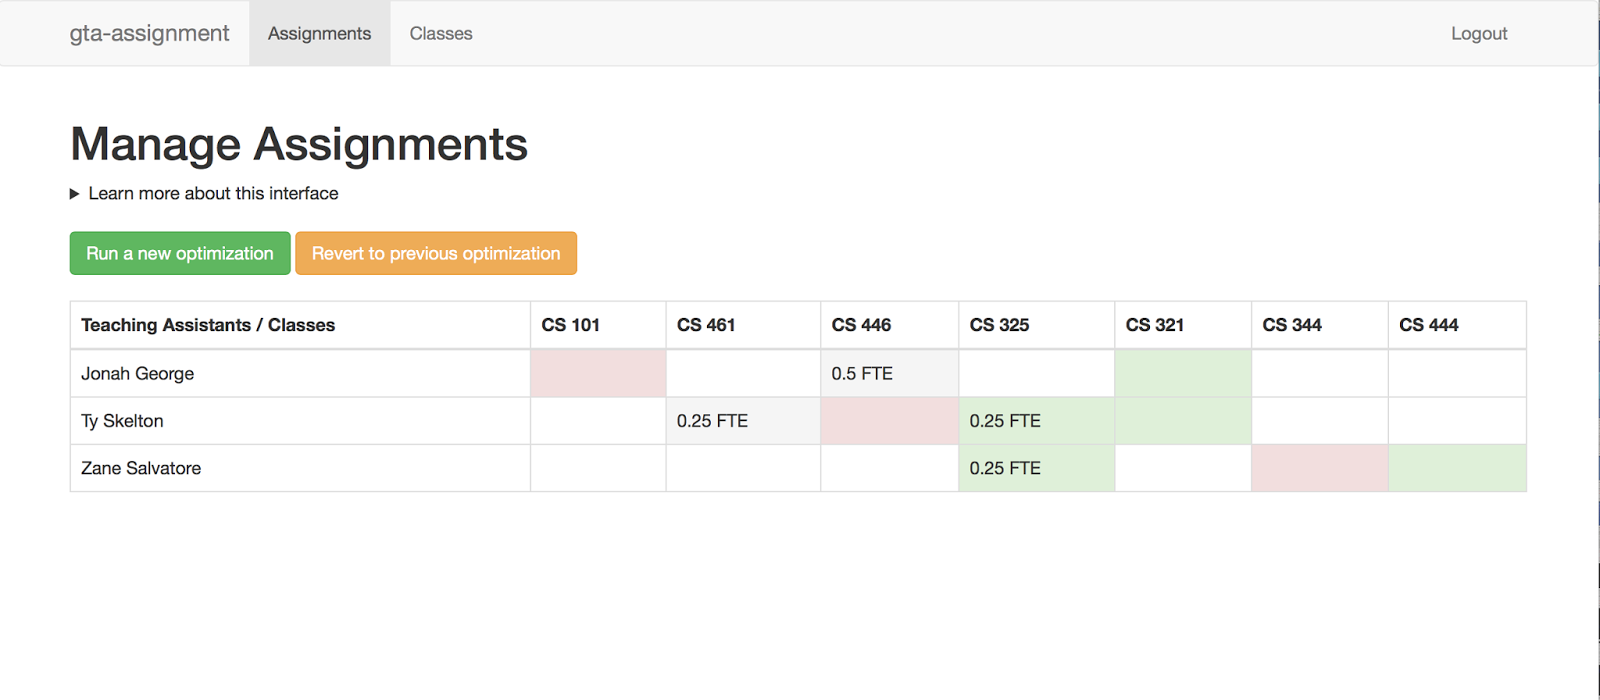
\includegraphics[width=0.75\linewidth]{images/administrator-assignment-design.png}
  \caption{Mock Admin Assignment Page}
\end{figure}

\begin{figure}[!htb]
  \centering
  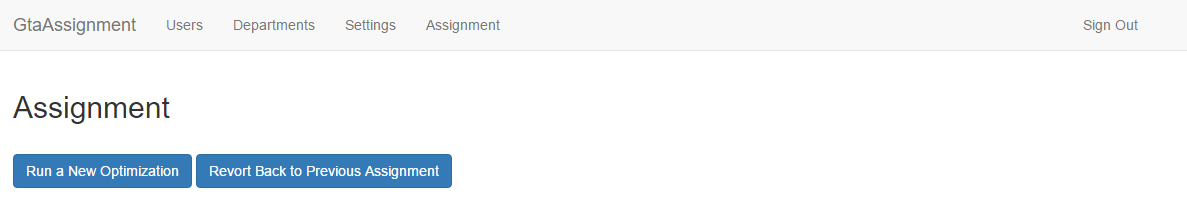
\includegraphics[width=0.75\linewidth]{images/administrator-assignment-alpha.png}
  \caption{Alpha Admin Assignment Page}
\end{figure}

\begin{figure}[!htb]
  \centering
  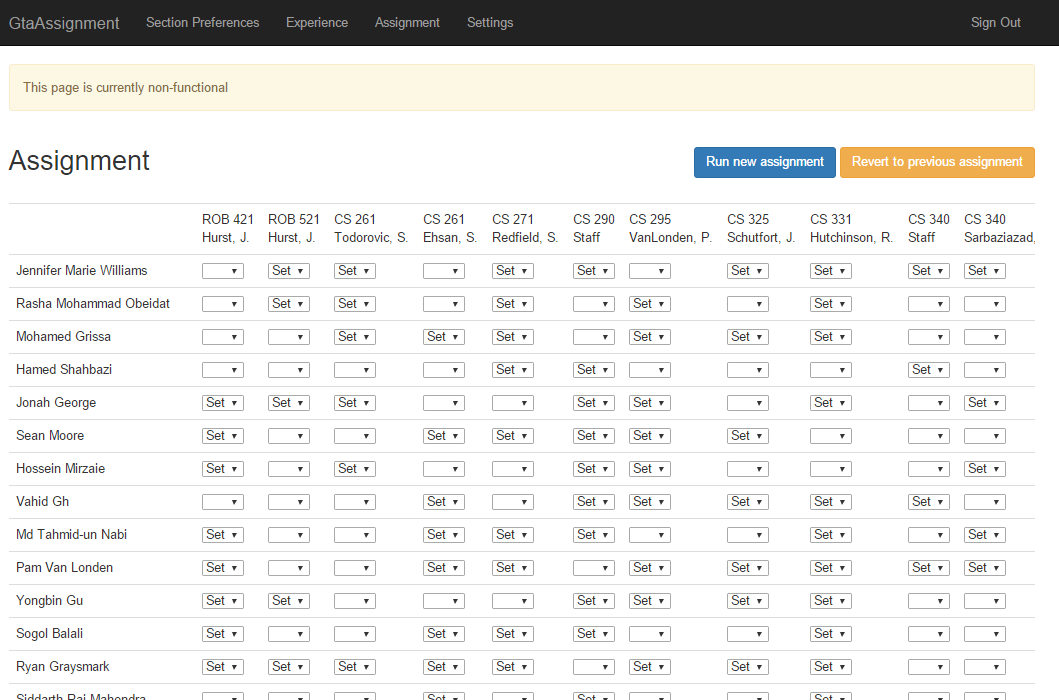
\includegraphics[width=0.75\linewidth]{images/administrator-assignment-beta.png}
  \caption{Beta Admin Assignment Page}
\end{figure}

\begin{figure}[!htb]
  \centering
  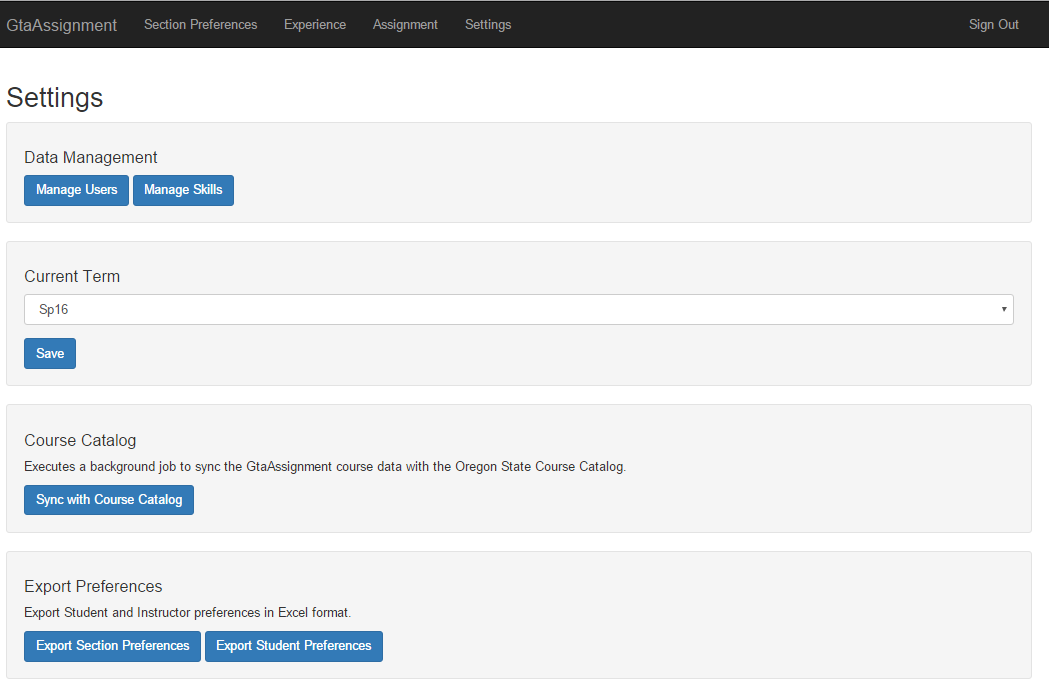
\includegraphics[width=0.75\linewidth]{images/administrator-settings-beta.png}
  \caption{Release Admin Settings Page}
\end{figure}

% \begin{figure}[!htb]
%   \centering
%   \minipage{0.5\textwidth}
%     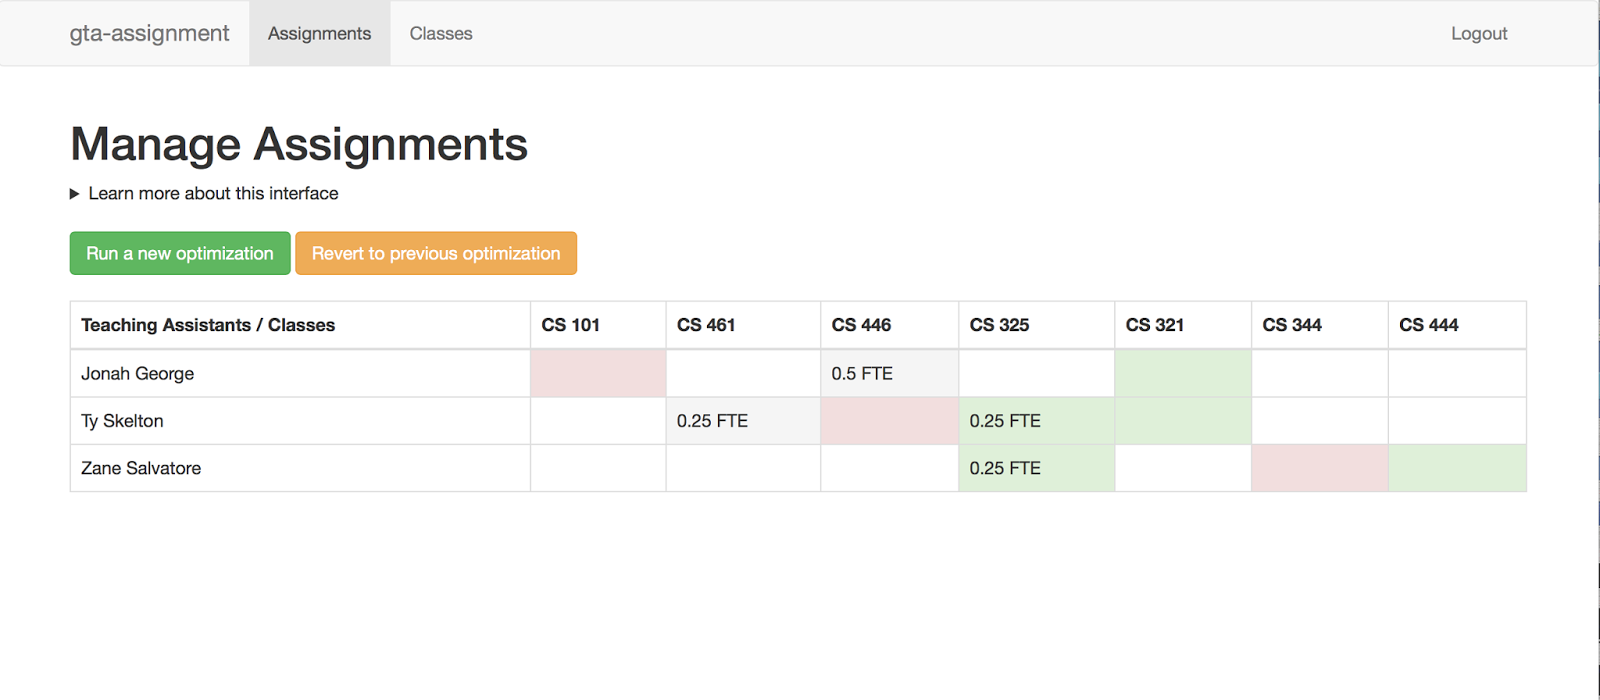
\includegraphics[width=\linewidth]{images/administrator-assignment-design.png}
%     \caption{Mock Admin Assignment Page}
%   \endminipage\hfill
%   \minipage{0.5\textwidth}
%     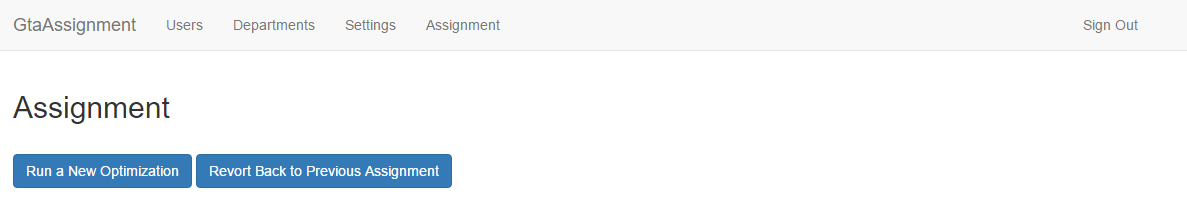
\includegraphics[width=\linewidth]{images/administrator-assignment-alpha.png}
%     \caption{Alpha Admin Assignment Page}
%   \endminipage\hfill
%   \minipage{0.5\textwidth}
%     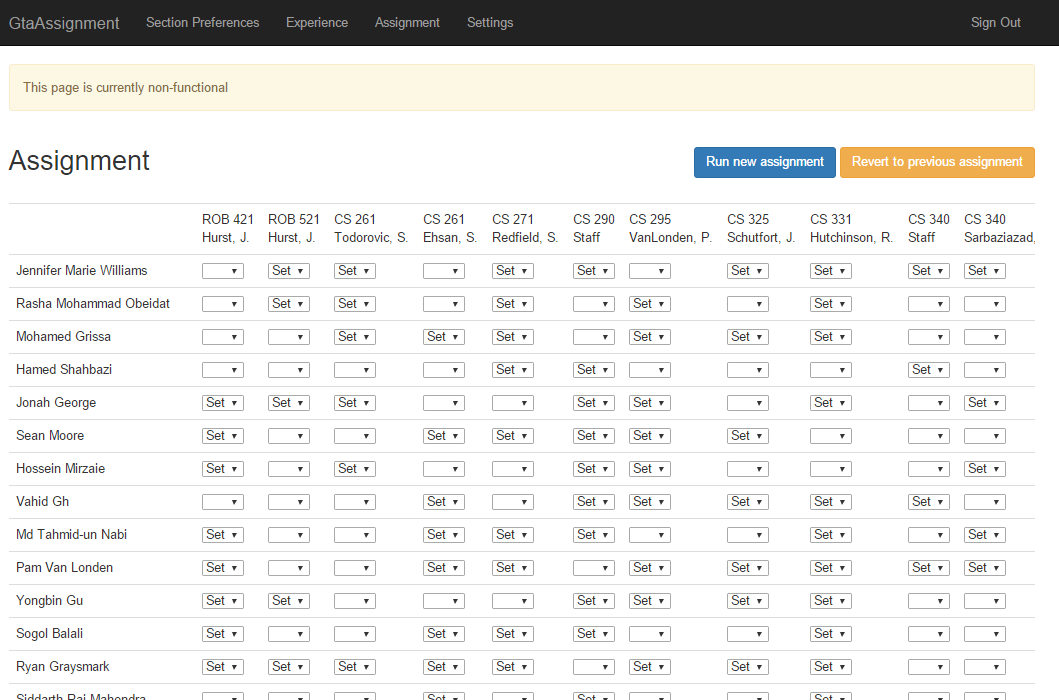
\includegraphics[width=\linewidth]{images/administrator-assignment-beta.png}
%     \caption{Beta Admin Assignment Page}
%   \endminipage\hfill
%   \minipage{0.5\textwidth}
%   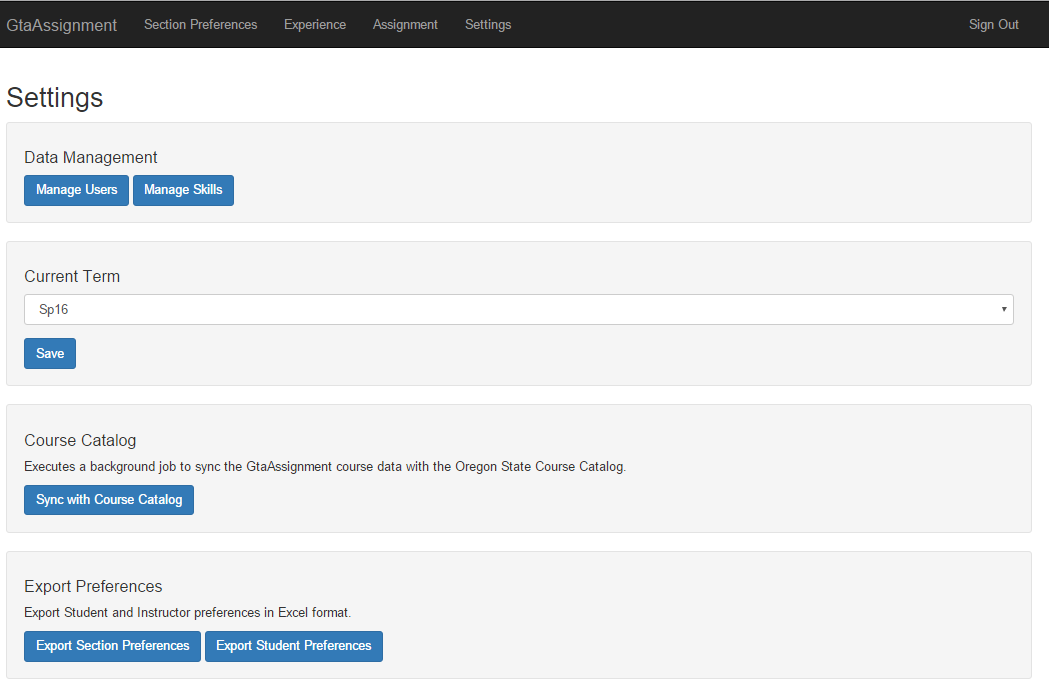
\includegraphics[width=\linewidth]{images/administrator-settings-beta.png}
%   \caption{Release Admin Settings Page}
%   \endminipage\hfill
% \end{figure}

The administrator pages is where most of the action happens.
The administrators have the power to hard code certain students to classes, export both student and instructors preferences.
Administrators also have access to advanced features like manual user and skill management and the ability to re-sync the site with the OSU Course Catalog.
Administrators are an integral part in the whole process- their prior knowledge from assigning TAs to courses will be key in making sure everyone is happy with the results after the ILP has done the heavy-lifting.

Like we pointed out above, the manage users feature has been moved from their the administrators can still modify users like changing their full-time equivalence (FTE) or promoting users to administrator status.
The Current Term field allows the administrators to select the current term which scopes the sections shown throughout the entire site.
The Course Catalog Sync button will trigger a background job update this system's data straight from the OSU Course Catalog.
Finally, the administrators can export the student and instructor preferences to Excel format to be used for reconciling assignment if needed.

\begin{figure}[!htb]
  \centering
  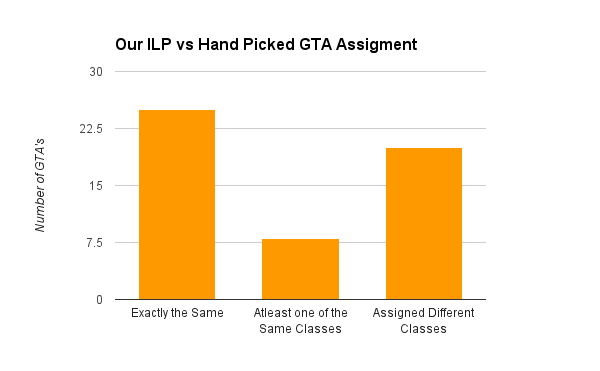
\includegraphics[width=0.75\linewidth]{images/ILPResults.png}
  \centering
  \caption{Our ILP Results vs Hand Picked Results for Winter 2016}\label{ILPresults}
\end{figure}

Using data from the Winter 2016 batch of graduate teaching assistants, we were able to compare the hand picked solution with our LP solution.
A good comparison graph can be seen in figure \ref{ILPresults}.
Our LP was able to assign the exact same class 47.2\% percent of time while also assigning the same class plus another class 15.1\%.
When our algorithm selected different classes, it usually selected students first or second choice 60\% of the time, meaning it was a matter of judgment on the part of those hand picking.
While 37.7\% different assignment might seem high, it is a good result given that there are real world constraints that our system may not capture, e.g. social factors and funding sources.

\subsection{Interesting Code}

Of all the interesting code in this project, there are two pieces that stand out.
Particularly, the backgrounds job associated with syncing the applications data with the data in the OSU Course Catalog and the code used to model the integer linear program.
First focusing on the background job code, we are using the ActiveJob interface from Ruby on Rails to define a background job that is run by the DelayedJob adapter.
This implements a queue using a table in Postgres through which a secondary "worker" process will pop jobs off and execute them.
The code included below is the "CourseSyncJob", the second of three background job.
It takes all of the departments declared on the OSU Course Catalog and scrapes it to find each of the department's courses.
These courses are compared to the ones already saved in the database.
If a new course is detected, an object is constructed and saved.
If not, the existing object is updated with any new values that came from the Course Catalog.

\begin{lstlisting}
class CoursesSyncJob < ActiveJob::Base
  queue_as :default

  def perform(department_id, cc_department_json)
    cc_department = OsuCcScraper::Department.from_json(cc_department_json)

    cc_courses(cc_department).each do |cc_course|
      course = Course.find_or_create_by(
        department_id: department_id, course_number: cc_course.course_number)
      course.update_attributes(name: cc_course.name)
      course.save

      SectionsSyncJob.perform_later(course.id, cc_course.to_json)
    end
  end

  private

    def cc_courses(cc_department)
      cc_department.courses.select { |c|
        course_whitelist.include?("#{cc_department.subject_code} #{c.course_number}")
      }
    end

    def course_whitelist
      ["CS 225", "CS 261", "CS 261", "CS 271", "CS 290"]
    end
end
\end{lstlisting}

The second piece of interesting code is a class called \textit{IntegerLinearProgram}.
This class encapsulates all of the logic necessary to model the ILP.
It uses a third-party library called "rulp" to handle the actual Ruby domain-specific language (DSL) to linear-program (LP) modelling language conversion.
In this case, the class constructor takes two ActiveRecord (Ruby on Rails ORM) relations, "students" and "sections" and will query for additional data off of them.
Using this method, we can pass a subset of the students and sections in the system into the IntegerLinearProgram class and treat it as a "blackbox" solution as it will fetch whatever other data it requires.
After constructing all of the constraints in the class constructor, the programmer can call "solve" on the object which serializes the linear program to a string which is passed into the COIN-OR CBC solver.
The results is passed back to Ruby where it is re-serialized into Ruby objects that we can use in other parts of the system.

Because of the size of this class, it has been shortened to show the structure and we'll descend into a few particularly interesting methods. The structure of \textit{IntegerLinearProgram} is as follows:

\begin{lstlisting}
class IntegerLinearProgram

  def initialize(students, sections, fixed_assignments = {}, fte_per_section = 0.25, students_per_ta = 30)
    @students = students
    @sections = sections
    @fixed_assignments = fixed_assignments
    @fte_per_section = fte_per_section
    @students_per_ta = students_per_ta

    @problem = Rulp::Max(objective)
    enrollment_contraint
    fte_contraint
    skill_contraint
    fixed_assignments_constraint if @fixed_assignments
  end

  def solve; end
  def results; end
  def print_results; end

private

  def objective; end
  def enrollment_contraint; end
  def fte_contraint; end
  def skill_contraint; end
  def fixed_assignments_constraint; end

end
\end{lstlisting}

The first interesting method is the \textit{objective} method.
This method is responsible for modelling the objective function of the linear program.
It starts by iterating all of the sections to build a hashmap of the instructor's preferences of students.
The keys of this hash are a combination of the student's id and the section's id.

Next, it starts iterating student-by-student building the linear program variables.
First, it builds a similar hashmap structure for student preference's of sections.
Then starts iterating section-by-section retrieving the student's preference of the section and the instructor's preference of the student for said section.
If either of these values does not exist, it substitutes a value of \textit{1}.
Finally, it builds an array of these LP variables in the \textit{variables} variable.
At the end, \textit{variables} is summed and returned.

\begin{lstlisting}
def objective
  variables = []

  instructor_student_preferences = {}
  @sections.each do |section|
    if section.instructor
      section.instructor.student_preferences.each do |preference|
        instructor_student_preferences[:"#{preference.student.id}_#{section.id}"] = preference
      end
    end
  end

  @students.each do |student|
    section_preferences =
      student.section_preferences.index_by { |preference| :"#{student.id}_#{preference.section.id}" }

    @sections.each do |section|
      student_score = section_preferences[:"#{student.id}_#{section.id}"].try(:value_raw)
      student_score ||= 1

      instructor_score = instructor_student_preferences[:"#{student.id}_#{section.id}"].try(:value_raw)
      instructor_score ||= 1

      variables << (student_score * instructor_score * VAR_b(student.id, section.id))
    end
  end
  variables.sum
end
\end{lstlisting}

The second piece of interesting code is the \textit{skill\_constraint} method.
This is one of the four constraints that are programmed into our linear program.
This one in particular is responsible for preventing teaching assistants from being assigned to classes that they are not qualified to TA.
Similar to the objective function, it starts iterating student-by-student and building a hashmap of experience records.
Then, it iterates by sections and the requirements for each section to determine which constraints need to be added.
If a section has a particular requirement and the student does not fulfill that requirement, a "hard" constraint settings the value to zero is added to the linear program.

\begin{lstlisting}
def skill_contraint
  @students.each do |student|
    experiences = student.experiences.index_by { |experience| :"#{experience.skill_id}" }

    @sections.each do |section|
      section.course.requirements.each do |requirement|
        exp = experiences[:"#{requirement.skill_id}"]
        if exp == nil || exp[:value] < requirement[:value]
          @problem[ VAR_b(student.id, section.id) <= 0 ] # Hardcode to NO
        end
      end
    end
  end
end
\end{lstlisting}

\subsection{Future Work}

\subsubsection{Allow For Re-Loading of Prior Assigments}

One of the last requirments we need to fill is to allow for assignments to be re-loaded into the system from previous iterations.
Creating a section in our Database with the results of ILP and being able to translate into viewable content is our next challenge.

\subsubsection{Continue with User Testing}

We will continue to have both instructors and students use the site so that we can listen to their feedback.
Currently, we have been hearing good things from both of our users after some minor changes in the past couple of months.
The goal is to send out a survey to both instructors and students with our ILP results vs the hand assigned solution.
The survey will also ask them about their experience using the site.

\subsubsection{Timeline}

\begin{center}
  \begin{tabular}{| l | l |}
  \hline
  Spring, Week 6      & Continue listening to feedback from users. \\ \hline
  Spring, Week 7      & Allow for saving and reloading of prior assigments. \\ \hline
  Spring, Week 8      & Engineering Expo, have finished product ready. \\ \hline
  Spring, Week 9 - 10 & Meet with sponsor to go over final product. \\ \hline
  \end{tabular}
\end{center}


\end{document}
